\section{ĐƯỜNG TRÒN} % Tên bài
\subsection{KIẾN THỨC TRỌNG TÂM}
\subsubsection{Khái niệm đường tròn}
	Đường tròn tâm $O$ bán kính $R$ ($R>0$), kí hiệu $(O;R)$, là hình gồm tất cả các điểm trong mặt phẳng cách $O$ một khoảng bằng $R$.
\begin{luuy}
	Khi không cần chú ý đến bán kính, đường tròn $(O;R)$ còn được kí hiệu là $(O)$.
\end{luuy}

\begin{nx}
\begin{enumerate}
	\item Cho điểm $M$ và đường tròn $(O, R)$. Khi đó
	\begin{enumerate}
		\item Nếu $OM=R$ thì $M$ nằm trên đường tròn hay $M$ thuộc đường tròn, ta viết $M \in (O)$.
		\item Nếu $OM<R$ thì $M$ nằm trong đường tròn.
		\item Nếu $OM>R$ thì $M$ nằm ngoài đường tròn.
	\end{enumerate}
	\begin{center}
		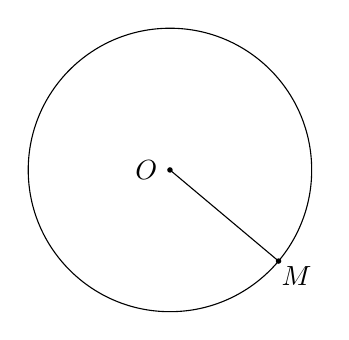
\begin{tikzpicture}
			\def\r{2}
			\path 
			(0,0) coordinate (O)
			(-40:1.8) coordinate (M);
			\draw (0,0) circle (1.8);
			\draw (O)--(M);
			\foreach \p/\r in {M/-40,O/180}
			\fill (\p) circle (1pt) node[shift={(\r:3mm)}]{$\p$};
		\end{tikzpicture} \qquad 
		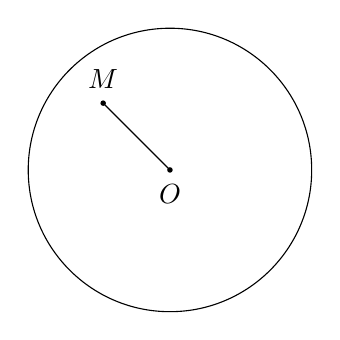
\begin{tikzpicture}
			\def\r{2}
			\path 
			(0,0) coordinate (O)
			(135:1.2) coordinate (M);
			\draw (0,0) circle (1.8);
			%		\draw (0,-2) node[below]{b)};
			%	\draw (-2,-3) node[below]{Hình $2$};
			\draw (O)--(M);
			\foreach \p/\r in {M/90,O/-90}
			\fill (\p) circle (1pt) node[shift={(\r:3mm)}]{$\p$};
		\end{tikzpicture} \qquad 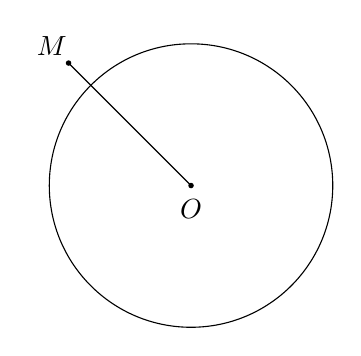
\begin{tikzpicture}
			\def\r{2}
			\path 
			(0,0) coordinate (O)
			(135:2.2) coordinate (M);
			\draw (0,0) circle (1.8);
			\draw (O)--(M);
			\foreach \p/\r in {M/135,O/-90}
			\fill (\p) circle (1pt) node[shift={(\r:3mm)}]{$\p$};
		\end{tikzpicture}
	\end{center}
	\item Hình tròn tâm $O$ bán kính $R$ là hình gồm các điểm nằm trên và nằm trong đường tròn $(O,R)$.
\end{enumerate}
\end{nx}

\subsubsection{Tính đối xứng của đường tròn}

\begin{enumerate}
	\item Đường tròn là hình có tâm đối xứng; tâm đối xứng là tâm của đường tròn.
	\item Đường tròn là hìnhcó trục đối xứng. Mọi đường thẳng đi qua tâm của đường tròn đều là trục đối xứng của nó.
\end{enumerate}

\subsubsection{Đường kính và dây cung của đường tròn}

\begin{enumerate}
	\item Đoạn thẳng nối hai điểm phân biệt thuộc hai điểm phân biệt thuộc đường tròn được gọi là dây (hoặc dây cung) của đường tròn.
	\item Đường kính là một dây đi qua tâm.
	\item Trong các dây của một đường tròn, đường kính là dây cung có độ dài lớn nhất.
\end{enumerate}

\subsubsection{Vị trí tương đối của hai đường tròn}
Cho hai đường tròn phân biệt $(O; R)$ và $(O'; R')$ với $R\ne R'$. Khi đó
\begin{center}
\begin{tabular}{|m{6cm}|c|c|m{3.5cm}|}
	\hline
	\textbf{Vị trí tương đối}  & \textbf{Số điểm chung} &\textbf{ Hệ thức liên 
		hệ} & \textbf{Hình ảnh} \\
	\hline
	Hai đường tròn cắt nhau& 2 & $|R-R'|<OO'<R+R'$ & \qquad
	\begin{tikzpicture}
		\path
		(0,0) coordinate (O)
		(1.4,0) coordinate (O')
		;
		\draw [name path=dgtronO,samples=200,smooth] (O) circle 
		(1); 
		\draw [name path=dgtronO',samples=200,smooth](O') circle 
		(0.65);
		\path[name intersections={of=dgtronO and dgtronO'}]
		(intersection-1) coordinate (A)
		(intersection-2) coordinate (B);
		\draw[samples=200,smooth] (A)--(B) (O)--(O');
		\foreach \q/\r in{A/85,B/-90,O/-90,O'/-90}
		\fill (\q) circle (1pt) node[shift={(\r:3.5mm)}]{$\q$};
	\end{tikzpicture}	 \\
	\hline
	Hai đường tròn tiếp xúc ngoài &1  & $OO'=R+R'$ & \qquad
	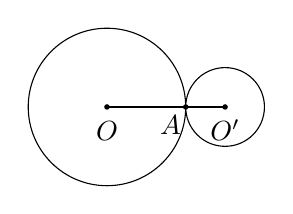
\begin{tikzpicture}
		\path
		(0,0) coordinate (O)
		(1.5,0) coordinate (O')
		(1,0) coordinate (A);
		\draw [samples=200,smooth] (O) circle (1) 
		(O') circle (0.5);
		\draw (O)--(O');
		\foreach \p/\r in{O/-90,O'/-90,A/-130}
		\fill (\p) circle (1pt) node[shift={(\r:3mm)}]{$\p$};
		
	\end{tikzpicture} \\
	\hline
	Hai đường tròn tiếp xúc trong &1  & $OO'=|R-R'|$ &\qquad
	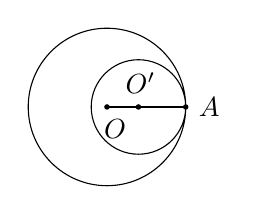
\begin{tikzpicture}
		\path
		(0,0) coordinate (O)
		(0.4,0) coordinate (O')
		(1,0) coordinate (A);
		\draw [samples=200,smooth] (O) circle (1) 
		(O') circle (0.6);
		\draw (O)--(A);
		\foreach \p/\r in{O/-70,O'/85,A/0}
		\fill (\p) circle (1pt) node[shift={(\r:3mm)}]{$\p$};
		
	\end{tikzpicture}  \\
	\hline
	Hai đường tròn ở ngoài nhau & 0 &$OO'>R+R'$  & \qquad
	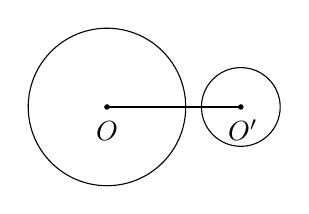
\begin{tikzpicture}
		\path
		(0,0) coordinate (O)
		(1.7,0) coordinate (O');
		\draw [samples=200,smooth] (O) circle (1) 
		(O') circle (0.5);
		\draw (O)--(O');
		\foreach \p/\r in{O/-90,O'/-85}
		\fill (\p) circle (1pt) node[shift={(\r:3mm)}]{$\p$};
		
	\end{tikzpicture} \\
	\hline
	Đường tròn $(O;R)$ đựng đường tròn $(O';R')$& $0$ &  $OO'<|R-R'|$ & \qquad
	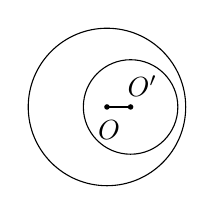
\begin{tikzpicture}
		\path
		(0,0) coordinate (O)
		(0.3,0) coordinate (O');
		\draw [samples=200,smooth] (O) circle (1) 
		(O') circle (0.6);
		\draw (O)--(O');
		\foreach \p/\r in{O/-85,O'/60}
		\fill (\p) circle (1pt) node[shift={(\r:3mm)}]{$\p$};
	\end{tikzpicture} \\
	\hline
\end{tabular}
\end{center}

\subsection{CÁC DẠNG BÀI TẬP}

\begin{dang}{Xác định vị trí tương đối của điểm đối với đường tròn}
\end{dang}

\begin{vd}%[Dự án EX-9-Đề Cương Toán 9]%[Trần Chiến]%[9H2H1-1]
	Cho đường tròn $(O)$, bán kính $4$ cm và bốn điểm $A$, $B$, $C$, $D$ thỏa mãn $OA=3$ cm, $OB=4$ cm, $OC=6$ cm, $OD=5$ cm. Hãy cho biết mỗi điểm $A$, $B$, $C$, $D$ nằm trong, nằm trên hay nằm ngoài đường tròn $(O)$.
\loigiai{
	\begin{enumerate}
		\item $OA=3<R=4$ nên điểm $A$ ở trong đường tròn.
		\item $OB=4=R=4$ nên điểm $B$ ở trên đường tròn.
		\item $OC=7>R=4$ nên điểm $C$ ở ngoài đường tròn.
		\item $OD=5>R=4$ nên điểm $D$ ở ngoài đường tròn.
	\end{enumerate}
}
\end{vd}

\begin{vd}%[Dự án EX-9-Đề Cương Toán 9]%[Trần Chiến]%[9H2H1-1]
	Cho tam giác đều $ABC$ có cạnh bằng $2$. Gọi $M$, $K$, $N$ lần lượt là trung điểm của đoạn $AB$, $BC$, $AC$ và $G$ là trọng tâm tam giác $ABC$. Vẽ đường tròn đường kính $BC$. Hãy cho biết mỗi điểm $A$, $M$, $N$, $G$ nằm trong, nằm trên hay nằm ngoài đường tròn đường kính $BC$.
\loigiai{
\begin{center}
\begin{tikzpicture}[scale=1, line join=round, line cap=round, >=stealth]
	\coordinate (B) at (0,0);
	\coordinate (C) at (4,0);
	\coordinate (A) at ($(B)!1!60:(C)$);
	\coordinate (M) at ($(A)!0.5!(B)$);
	\coordinate (K) at ($(C)!0.5!(B)$);
	\coordinate (N) at ($(A)!0.5!(C)$);
	\coordinate (G) at ($(A)!2/3!(K)$);
	\draw (A)--(B)--(C)--cycle
	(A)--(K)--(M) (N)--(K)
	;
	\draw[name path=o] (K) let \p1=($(K)-(C)$) in circle ({veclen(\x1,\y1)});
	\foreach \i/\j in {A/90,B/-140,C/-40,M/150,K/-90,N/30,G/0} \fill[black] (\i) circle (1pt) ($(\i)+(\j:3mm)$)node{$\i$};
	\end{tikzpicture}
\end{center}
	Do $K$ là trung điểm của $BC$ nên $K$ là tâm của đường tròn đường kính $BC$, bán kính đường tròn là $R=\dfrac{BC}{2} =1$.\\
	Do $MK$ và $NK$ là các đường trung bình của tam giác $ABC$ nên $MK=NK=1=R$. Suy ra $M$, $N$ thuộc đường tròn đường kính $BC$.\\
	Do $\triangle ABC$ đều và $AK$ là đường trung tuyến nên $AK \perp BC$. \\
	Xét tam giác $ABK$ vuông tại $K$ ta có
	\\
	$AK=\sqrt{AC^2-KC^2}=\sqrt{2^2-1^2}=\sqrt{3}>R$, suy ra điểm $A$ nằm ngoài đường tròn đường kính $BC$.\\
	Do $G$ là trọng tâm tam giác $ABC$ nên $GK=\dfrac{1}{3}AK =\dfrac{\sqrt{3}}{3} <R$, suy ra điểm $G$ nằm trong đường tròn đường kính $BC$.
	}
\end{vd}


\begin{dang}{Chứng minh nhiều điểm cùng thuộc một đường tròn}
\end{dang}

\begin{vd}%[Dự án EX-9-Đề Cương Toán 9]%[Trần Chiến]%[9H2H1-1]
	Cho hình chữ nhật $ABCD$ có $AD=9$ cm và $CD=6$ cm. Chứng minh rằng bốn điểm $A$, $B$, $C$, $D$ cùng thuộc một đường tròn. Tính bán kính của đường tròn đó.
\loigiai{
\immini{
	Gọi $O$ là tâm của hình chữ nhật, suy ra $OA=OB=OC=OD$.\\
	Vì vậy các điểm $A$, $B$, $C$, $D$ nằm trên một đường tròn tâm $O$, bán kính $OA$.\\
	Tam giác $ABC$ vuông tại $B$ có  $$AC=\sqrt{AB^2+BC^2}=\sqrt{6^2+9^2}=\sqrt{117} \text{ (cm)}.$$
	Vậy bán kính $R=\dfrac{AC}{2}=\dfrac{\sqrt{117}}{2}$ (cm).
}{
\begin{tikzpicture}[scale=1, line join=round, line cap=round, >=stealth]
	\path
	(0,0) coordinate (B)
	(3,0) coordinate (C)
	(0,2) coordinate (A)
	(3,2) coordinate (D)
	($(D)!0.5!(B)$)coordinate (O);
	\draw (O) let \p1=($(O)-(B)$) in circle ({veclen(\x1,\y1)});
	\draw 
	(A)--(B)--(C)--(D)--(A) ;
	\foreach \x/\g in {A/150,B/210,C/-20,D/40,O/-90}
	\draw [fill=black] (\x) circle (1pt)+(\g:.3) node{$\x$};
\end{tikzpicture}
}
}
\end{vd}

\begin{vd}%[Dự án EX-9-Đề Cương Toán 9]%[Trần Chiến]%[9H2H1-1]	
	Cho tứ giác $ABCD$ có hai đường chéo vuông góc với nhau. Gọi $M$, $N$, $P$, $Q$ lần lượt là trung điểm của các cạnh $AB$, $BC$, $CD$ và $AD$. Chứng minh rằng bốn điểm $M$, $N$, $P$, $Q$ cùng thuộc một đường tròn.
\loigiai{
\begin{center}
\begin{tikzpicture}[scale=1, line join=round, line cap=round, >=stealth]
	\coordinate (A) at (0,2);
	\coordinate (C) at (0,-3);
	\coordinate (B) at (-3,0);
	\coordinate (D) at (4,0);
	\coordinate (M) at ($(A)!0.5!(B)$);
	\coordinate (N) at ($(C)!0.5!(B)$);
	\coordinate (P) at ($(C)!0.5!(D)$);
	\coordinate (Q) at ($(A)!0.5!(D)$);
	\coordinate (O) at ($(M)!0.5!(P)$);
	\coordinate (I) at (intersection of A--C and B--D);
	\draw (A)--(B)--(C)--(D)--cycle
	(A)--(C) (B)--(D)
	(M)--(N)--(P)--(Q)--cycle
	;
	\draw[dashed] (O) let \p1=($(O)-(M)$) in circle ({veclen(\x1,\y1)});
	\draw pic[draw, angle radius=2mm]{right angle=D--I--A};
	\foreach \i/\j in {A/90,B/-90,C/180,D/0,M/120,N/-120,P/-60,Q/60,O/-30}
	\fill[black] (\i) circle (1pt) ($(\i)+(\j:3mm)$)node{$\i$};
	\end{tikzpicture}
\end{center}
	Xét tam giác $ABD$ có $M$ và $Q$ lần lượt là trung điểm của $AB$ và $AD$ nên $MQ$ là đường trung bình. Suy ra $MQ \parallel BD$ và $MQ=\dfrac{1}{2}BD \qquad (1)$.\\
	Xét tam giác $CBD$ có $N$ và $P$ lần lượt là trung điểm của $CB$ và $CD$ nên $NP$ là đường trung bình. Suy ra $NP \parallel BD$ và $NP=\dfrac{1}{2}BD \qquad (2)$.\\	
	Từ $(1)$ và $(2)$ suy ra $MQ \parallel NP$ và $MQ=NP$. Vì vậy tứ giác $MQNP$ là hình bình hành $(3)$.\\
	Tương tự ta có $MN$ là đường trung bình của tam giác $ABC$, suy ra $MN \parallel AC$.\\
	Do $MN \parallel AC$,  $MQ \parallel BD$ và $AC \perp BD$ nên $MQ \perp MN$. Suy ra $\widehat{NMQ}=90^\circ$ $(4)$.\\
	Từ $(3)$ và $(4)$ suy ra tứ giác $MNPQ$ là hình chữ nhật. \\
	Gọi $O$ là tâm của hình chữ nhật, suy ra $OM=ON=OP=OQ$.\\
	Vì vậy các điểm $M$, $N$, $P$, $Q$ nằm trên một đường tròn tâm $O$, bán kính $OM$.
}
\end{vd}


\begin{dang}{Tâm đối xứng và trục đối xứng của đường tròn}
\end{dang}

\begin{vd}%[Dự án EX-9-Đề Cương Toán 9]%[Trần Chiến]%[9H2N1-2]
	Trên đường tròn $(O;R)$ lấy hai điểm $M$ và $M'$ nằm trên đường tròn. Gọi $d$ là đường thẳng đi qua tâm $O$ và vuông góc với $MM'$.
	\begin{enumerate}
		\item Chứng minh $d$ là trung trực của $MM'$.
		\item Điểm $N$ thuộc đường tròn, lấy $N'$ đối xứng với $N$ qua $d$. Chứng minh $N'$ nằm trên đường tròn. 
	\end{enumerate} 
\loigiai{
\begin{center}
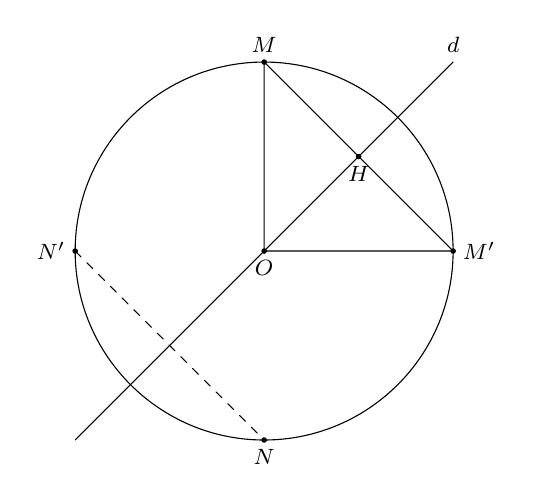
\begin{tikzpicture}[scale=0.8, font=\footnotesize, line join=round, line cap=round, >=stealth]
	\draw (0,0) circle (3cm);
	\filldraw (0,0) circle (1pt) node[below] {$O$};
	\filldraw (0,3) circle (1pt) node[above] {$M$};
	\filldraw (3,0) circle (1pt) node[right] {$M'$};
	\filldraw (0,-3) circle (1pt) node[below] {$N$};
	\filldraw (-3,0) circle (1pt) node[left] {$N'$};
	\filldraw (1.5,1.5) circle (1pt) node[below] {$H$};
	\draw (3,0) -- (0,3)--(0,0)--(3,0);
	\draw (-3,-3) -- (3,3);
	\draw[dashed] (-3,0)--(0,-3);
	\node[above] at (3,3) {$d$};
\end{tikzpicture}
\end{center}
\begin{enumerate}
	\item Gọi $H$ là giao điểm của $d$ và $MM'$, suy ra $OH \perp MM'$.\\
	Xét tam giác $OMM'$ có $OM=OM'=R$ nên $\triangle OMM'$ cân tại $O$. Lại có $OH$ là đường cao nên $OH$ là đường trung trực của $MM'$, hay $d$ là đường trung trực cuả $MM'$.
	\item Do $d$ là đường thẳng đi qua tâm $O$ nên $d$ là trục đối xứng của đường tròn $(O)$. Mà $N'$ là điểm đối xứng của $N$ qua $d$ nên $N'$ thuộc đường tròn $(O)$.
\end{enumerate}	
}
\end{vd}


\begin{dang}{Liên hệ giữa đường kính và dây cung của đường tròn}
\end{dang}

\begin{vd}%[Dự án EX-9-Đề Cương Toán 9]%[Trần Chiến]%[9H2H1-3]
\immini{
	Cho đường tròn tâm $O$, bán kính $R=5$ và dây $AB=6$. Gọi $I$ là chân đường vuông góc kẻ từ $O$ đến $AB$, tia $OI$ cắt đường tròn tại $M$. Tính độ dài đoạn $AM$.
}{
\begin{tikzpicture}[scale=0.8, font=\footnotesize, line join=round, line cap=round, >=stealth]
	\coordinate (O) at (0,0);
	\draw[name path=c] (O) circle (3cm);
	\draw (O)++(0:3) coordinate (B);
	\draw (O)++(-90:3)coordinate (A);
	\coordinate (I) at ($(A)!0.5!(B)$);			
	\draw (A)--(B);
	\path[name path=x] (O)--($(O)!1.5!(I)$);
	\path [name intersections={of=c and x, by=M}];
	\draw (I)++(45:0.3)--++(135:0.3)--++(-135:0.3)
	(O)--(M) (A)--(O)--(B);
	\foreach \i/\j in {A/-90,B/0,M/-60,I/-90,O/90}
	\fill[black] (\i) circle (1pt) ($(\i)+(\j:3mm)$)node{$\i$};
\end{tikzpicture}
}
\loigiai{
	Xét tam giác $OAB$ có $OA=OB$ nên tam giác $OAB$ cân tại $A$.\\
	Mà $OI$ là đường cao của tam giác nên $OI$ là trung tuyến, suy ra $I$ là trung điểm $AB$.\\
	Suy ra $AI =\dfrac{AB}{2}=3$.\\
	Xét tam giác $OAI$ vuông tại $I$ có 
	$$OI=\sqrt{OA^2-AI^2}=\sqrt{{5^2}-{3^2}}=4.$$
	Ta có $MI=OM-OI=5-4=1$.\\
	Xét tam giác $AIM$ vuông tại $I$ có
	$$AM=\sqrt{A{I^2}+M{I^2}}=\sqrt{{3^2}+{1^2}}=\sqrt{10}.$$
}
\end{vd}

\begin{vd}%[Dự án EX-9-Đề Cương Toán 9]%[Trần Chiến]%[9H2H1-3]
	Trong đường tròn $(O; R)$ có hai bán kính $OA$ và $OB$ sao cho $\widehat{AOB}=120^{\circ}$. Gọi $OI$ là đường cao của $\triangle {AOB}$. Tia $OI$ cắt đường tròn $(O)$ tại $C$.
	\begin{enumerate}
		\item  Tính độ dài cạnh $AB$, chiều cao $OI$ của $\triangle AOB$ theo $R$.
		\item  Chứng minh tứ giác $OACB$ là hình thoi. Tính diện tích của hình thoi $OACB$ theo $R$.
	\end{enumerate}
\loigiai{
\begin{enumerate}
	\item  
	\immini{
		Trong $\triangle ABO$ có $OA=OB=R$.\\
		Suy ra $\triangle ABO$ cân tại $O$. \\
		Mà  $OI$ là đường cao nên $OI$ cũng là đường phân giác, suy ra $\widehat{AOI}=\widehat{BOI}=\dfrac{1}{2}\cdot \widehat{AOB}=\dfrac{1}{2}\cdot 120^{\circ}=60^{\circ}$.\\
		Trong $\triangle AOI$ vuông tại $I$, ta có\\
		$AI=OA\cdot \sin 60^{\circ}=\dfrac{R\sqrt{3}}{2}$ và
		$OI=OA\cdot \cos 60^{\circ}=\dfrac{R}{2}$.\\
		Do $\triangle OAB$ cân tại $O$ và $OI$ là đường cao nên $I$ là trung điểm của $AB$. Suy ra $AB=2AI=R\sqrt{3}$.\\
	}{
		\begin{tikzpicture}[>=stealth,line join=round,line cap=round,font=\footnotesize,scale=1]
			\def\r{2.5}
			\coordinate (O) at (0,0);
			\coordinate (M) at (\r,0);
			\draw (O) circle(\r);
			\coordinate (A) at ($(O)!1!-150:(M)$);
			\coordinate (B) at ($(O)!1!-30:(M)$);
			\coordinate (I) at ($(A)!0.5!(B)$);
			\coordinate (x) at ($(O)!1!(I)$);
			\coordinate (C) at ($(O)!1!-90:(M)$);
			\draw (O)--(B)--(A)--(O)--(I)--(C) (A)--(C)--(B);
			\foreach \d/\g in {O/90, A/-150,B/-30,I/-45,C/-90} \fill (\d) circle(1pt) + (\g:.3) node{$\d$};
			\foreach \a/\b/\c in {O/I/A}{\draw pic[draw,angle radius=2mm] {right angle=\a--\b--\c};}
			\path (A)--(I) node[midway,sloped] {/};
			\path (B)--(I) node[midway,sloped] {/};
		\end{tikzpicture}
	}
	\item Do $OI=\dfrac{R}{2}$ nên $OI=\dfrac{OC}{2}$ hay $I$ là trung điểm của $OC$.\\
	Xét tứ giác $OACB$, ta có $OC\perp AB$ tại $I$, $IO=IC$ và $IA=IB$ nên  tứ giác $OACB$ là hình thoi.\\
	Diện tích hình thoi là $S_{OACB}=\dfrac{1}{2}\cdot OC\cdot AB=\dfrac{1}{2}\cdot R\cdot R\sqrt{3}=\dfrac{R^2\sqrt{3}}{2}$.
\end{enumerate}
}
\end{vd}


\begin{dang}{Vị trí tương đối của hai đường tròn}
\end{dang}

\begin{vd}%[Dự án EX-9-Đề Cương Toán 9]%[Trần Chiến]%[9H2N1-4]
	Tìm số điểm chung của hai đường tròn $(O)$ và $(O')$ trong mỗi trường hợp sau:
\begin{center}
	%hình a
	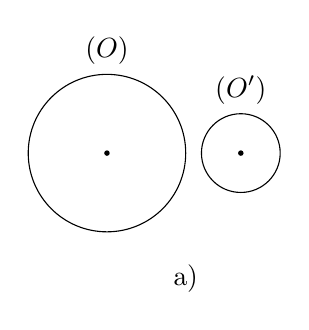
\begin{tikzpicture}[scale=1, line join=round, line cap=round, >=stealth]
		\path
		(0,0) coordinate (O)
		(1.7,0) coordinate (O');
		\draw [samples=200,smooth] (O) circle (1) 
		(O') circle (0.5);
		\draw (1,-1.3) node[below]{a)} (0,1) node[above]{$(O)$} (1.7,0.5) 
		node[above]{$(O')$};
		\foreach \p in{O, O'}
		\fill (\p) circle (1pt);
	\end{tikzpicture}
	\hspace{0.5cm}
	%hình b
	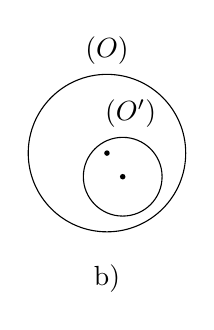
\begin{tikzpicture}[scale=1, line join=round, line cap=round, >=stealth]
		\path
		(0,0) coordinate (O)
		(0.2,-0.3) coordinate (O');
		\draw [samples=200,smooth] (O) circle (1) 
		(O') circle (0.5);
		\draw (0,-1.3) node[below]{b)} (0,1) node[above]{$(O)$} (0.3,0.2) 
		node[above]{$(O')$};
		\foreach \p in{O, O'}
		\fill (\p) circle (1pt);
	\end{tikzpicture}
	\hspace{0.5cm}
	%hình c
	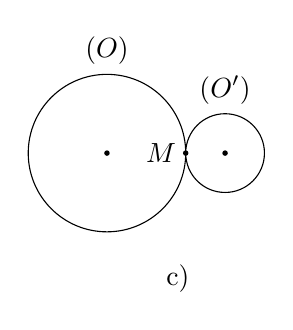
\begin{tikzpicture}[scale=1, line join=round, line cap=round, >=stealth]
		\path
		(0,0) coordinate (O)
		(1.5,0) coordinate (O')
		(1,0) coordinate (M);
		\draw [samples=200,smooth] (O) circle (1) 
		(O') circle (0.5);
		\draw (0.9,-1.3) node[below]{c)} (0,1) node[above]{$(O)$} (1.5,0.5) 
		node[above]{$(O')$} (1,0) node[left]{$M$};
		\foreach \p in{O, O',M}
		\fill (\p) circle (1pt);
	\end{tikzpicture}
	\hspace{0.5cm}
	%hình d
	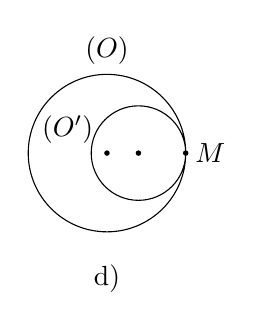
\begin{tikzpicture}[scale=1, line join=round, line cap=round, >=stealth]
		\path
		(0,0) coordinate (O)
		(0.4,0) coordinate (O')
		(1,0) coordinate (M);
		\draw [samples=200,smooth] (O) circle (1) 
		(O') circle (0.6);
		\draw (0,-1.3) node[below]{d)} (0,1) node[above]{$(O)$} (-0.5,0) 
		node[above]{$(O')$} (1,0) node[right]{$M$};
		\foreach \p in{O, O',M}
		\fill (\p) circle (1pt);
	\end{tikzpicture}
	\hspace{0.5cm}
	%hình e
	\begin{tikzpicture}[scale=1, line join=round, line cap=round, >=stealth]
		\path
		(0,0) coordinate (O)
		(1.4,0) coordinate (O')
		;
		\draw [name path=dgtronO,samples=200,smooth] (O) circle (1); 
		\draw [name path=dgtronO',samples=200,smooth](O') circle 
		(0.65);
		\path[name intersections={of=dgtronO and dgtronO'}]
		(intersection-1) coordinate (M)
		(intersection-2) coordinate (N);
		\draw (0.8,-1.3) node[below]{e)} (0,1) node[above]{$(O)$} (1.65,0.5) 
		node[above]{$(O')$};
		\foreach \p in{O, O',M}
		\fill (\p) circle (1pt);
		\foreach \q/\r in{M/80,N/-90}
		\fill (\q) circle (1pt) node[shift={(\r:4mm)}]{$\q$};
	\end{tikzpicture}
\end{center}
\loigiai{
	Dựa vào hình vẽ suy ra
	\begin{enumerate}
		\item Câu a) và b) số điểm chung của hai đường tròn là $0$.
		\item Câu c) và d) số điểm chung của hai đường tròn là $1$.
		\item Câu e) số điểm chung của hai đường tròn là $2$.
	\end{enumerate}
}
\end{vd}

\begin{vd}%[Dự án EX-9-Đề Cương Toán 9]%[Trần Chiến]%[9H2N1-4]
	Xác định vị trí tương đối giữa hai đường tròn $(I;R)$ và $(J;R')$ trong mỗi trường hợp sau
	\begin{enumerate}
		\item $IJ=5$; $R=3$; $R'=2$;
		\item $IJ=4$; $R=11$; $R'=7$;
		\item $IJ=6$; $R=9$; $R'=4$;
		\item $IJ=10$; $R=4$; $R'=1$.
	\end{enumerate}
\loigiai{
\begin{enumerate}
	\item Ta có $5=3+2$ nên $IJ'=R+R'$, suy ra hai đường tròn $(I;R)$ và $(J;R')$ tiếp xúc ngoài. 
	\item Ta có $4=11-7$ nên $IJ=R-R'$, suy ra đường tròn $(I;R)$ và $(J;R')$ tiếp xúc trong.
	\item Ta có $9-4<6<9+4$ nên $R-R'<IJ'<R+R'$, suy ra hai đường tròn $(I;R)$ và $(J ; R')$ cắt nhau.
	\item Ta có $10>4+1$ nên $IJ'>R+R'$, suy ra hai đường tròn $(I;R)$ và $(J;R')$ ở ngoài nhau.
\end{enumerate}
}
\end{vd}

\subsection{BÀI TẬP RÈN LUYỆN}

\begin{bt}%[Dự án EX-9-Đề Cương Toán 9]%[Trần Chiến]%[9H2H1-1]
	Cho hình thang cân $ABCD$ ($AD\parallel BC$) có $AD=2CD=2BC$. Chứng minh bốn điểm $A$, $B$, $C$, $D$ cùng nằm trên một đường tròn có tâm $O$ và $AC \perp OB$.
\loigiai{
\begin{center}
	\begin{tikzpicture}[scale=1, font=\footnotesize, line join=round, line cap=round, >=stealth]
		\def\R{2}
		\path
		(-\R,0) coordinate (A)
		(\R,0) coordinate (D)
		($ (A)+(60:\R) $) coordinate (B)
		($ (D)+(120:\R) $) coordinate (C)
		;		
		\draw (O) circle (\R);
		\draw (A)--(B)--(C)--(D)--cycle (A)--(C) (B)--(O) (O)--(C);
		\foreach \p/\r in {O/-90,A/180,B/120,C/60,D/-60}
		\fill (\p) circle (1pt) node[shift={(\r:3mm)}]{$\p$};
	\end{tikzpicture}
\end{center}
	Gọi $O$ là trung điểm $AD$. Khi đó $AO=DO=AB=CD=BC$.\\
	Xét hình thang $AOCB$ ta có $ \heva{& BC\parallel AO \\ & BC=AO}$ nên tứ giác $AOCB$ là hình bình hành.\\
	Chứng minh tương tự, ta có $DOBC$ là hình bình hành.\\
	Khi đó $ OA=OD=OB=OC=R $ nên $A$, $B$, $C$, $D$ cùng nằm trên một đường tròn có tâm $O$.\\
	Do $ABCO$ là hình bình hành nên $AB=OC=R$ nên $AB=AO$.\\
	Xét hình bình hành $ABCO$ có $AB=OC$ nên tứ giác $AOCB$ là hình thoi. Suy ra $AC\perp OB $.
}
\end{bt}

\begin{bt}%[Dự án EX-9-Đề Cương Toán 9]%[Trần Chiến]%[9H2V1-4]
	Trên đường thẳng $xy$, lấy lần lượt ba điểm $A$, $B$, $C$ sao cho $AB>BC$. Vẽ đường tròn $(O)$ đường kính $AB$ và đường tròn $(O')$ đường kính $BC$.
	\begin{enumerate}	
		\item  Chứng minh rằng hai đường tròn $(O)$ và $(O')$ tiếp xúc ngoài tại $B$.
		\item  Gọi $H$ là trung điểm của $AC$. Vẽ dây $DE$ của $(O)$ vuông góc với $AC$ tại $H$. Chứng minh tứ giác $ADCE$ là hình thoi.
		\end{enumerate}
\loigiai{
\begin{center}
	\begin{tikzpicture}[scale=1.4, line join=round, line cap=round, >=stealth]
		\path 
		(0,0)coordinate (x)+(0:8)coordinate (y)
		($(x)!.2!(y)$)coordinate (A) 
		($(x)!.8!(y)$)coordinate (C)
		($(A)!.6!(C)$)coordinate (B)
		($(B)!.5!(A)$)coordinate (O)
		($(B)!.5!(C)$)coordinate (O')
		($(A)!.5!(C)$)coordinate (H)
		($(H)+(90:2)$)coordinate (a)
		($(a)!2!(H)$)coordinate (b)
		;
		\path[name path=ab] (a)--(b);
		\draw[name path=circleO] let \p1=($(A)-(O)$) in (O) circle ({veclen(\x1,\y1)});
		\draw[name path=circleT] let \p1=($(B)-(O')$) in (O') circle ({veclen(\x1,\y1)});
		\path[name intersections={of= ab and circleO}] coordinate (E) at (intersection-1) coordinate (D) at (intersection-2);
		\path[name path=DC] (D)--(C);
		\path [name intersections={of=DC and circleT}]coordinate (F) at (intersection-2) 
		;
		\foreach \pointo/\pointt in {A/C,A/E,E/C,C/D,D/A,E/D,F/E,H/F,O'/F}{
			\draw[fill=black](\pointo)--(\pointt);
		}
		\foreach \point/\goc in {A/190,B/50,C/-10,H/150,D/-90,E/90,O/-90,O'/90}{
			\draw[fill=black](\point)circle(.8pt)+(\goc:2mm)node[scale=.8]{$\point$};
		}
	\end{tikzpicture}
\end{center}
\begin{enumerate}
	\item Đường tròn $(O)$ có bán kính $R_1=OB$, đường tròn $(O')$ có bán kính $R_2=O'B$.\\
	Khi đó $R_1+R_2=OB+O'B=OO'$, do đó hai đường tròn $(O)$ và $(O')$ tiếp xúc ngoài tại $B$.
	\item 
	Xét đường tròn $(O)$ có: $OE=OD$ (cùng bằng bán kính) $(1)$.\\
	Xét đường tròn $(O')$ có: $O'E=O'D$ (cùng bằng bán kính) $(2)$.\\
	Từ $(1)$ và $(2)$ suy ra $OO'$ là đường trung trực của đoạn $ED$. Vì vậy $H$ là trung điểm của $ED$.\\
	Lại có $H$ là trung điểm của $AC$, từ đó suy ra tứ giác $ADCE$ là hình bình hành.\\
	Mà hai đường chéo $AC$ và $DE$ vuông góc với nhau tại $H$ nên suy ra tứ giác $ADCE$ là hình thoi.
\end{enumerate}	
}
\end{bt}

\begin{bt}%[Dự án EX-9-Đề Cương Toán 9]%[Trần Chiến]%[9H2V1-1]
	Cho đoạn thẳng $AB=2a$ có trung điểm $O$. Trên đường trung trực của $AB$ lấy điểm $D$ sao cho $OD=\dfrac{a}{2}$. Nối $A$ với $D$, vẽ $BC$ vuông góc $AD$ tại $C$.
	\begin{enumerate}
		\item Tính $AD$, $AC$, $BC$ theo $a$.
		\item Trên tia đối của tia $OD$ lấy điểm $E$ sao cho $OE=a$. Chứng minh rằng bốn điểm $A$, $B$, $C$, $E$ cùng nằm trên một đường tròn và $CE$ là tia phân giác của $\widehat{ACB}$.
	\end{enumerate}
\loigiai{
\begin{center}
\begin{tikzpicture}[scale=1, font=\footnotesize, line join=round, line cap=round, >=stealth]
	\path
	(0,0) coordinate (A)
	(6,0) coordinate (B)
	($(A)!0.5!(B)$) coordinate (O)
	(3,1.5) coordinate (D)
	(3,-3) coordinate (E)
	($(A)!(B)!(D)$) coordinate (C)
	($(A)!(C)!(B)$) coordinate (I)
	;
	\draw 
	(A)--(E)--(B)--(C)--cycle
	(C)--(E)--(D)
	(A)--(B) (O)--(C) (C)--(I)
	;
	\foreach \p/\g in {A/170, B/0, C/90, D/90, O/-45, E/-45, I/-90}
	\draw[fill=black] (\p) circle (1pt) node[shift=(\g:3mm)] {$\p$};
	\pic[draw, angle radius=2mm] {right angle=A--C--B};
	\pic[draw, angle radius=2mm] {right angle=A--O--D};
	\pic[draw, angle radius=2mm] {right angle=C--I--B};
	\path (A)--(O) node[midway,sloped] {/};
	\path (B)--(O) node[midway,sloped] {/};
\end{tikzpicture}
\end{center}
\begin{enumerate}
	\item Tính $AD$, $AC$, $BC$ theo $a$.\\
	Tam giác $AOD$ vuông tại $O$ nên theo định lí Pythagore ta có\\ $AD^2=AO^2+DO^2=a^2+\left(\dfrac{a}{2}\right)^2=\dfrac{5a^2}{4}$, suy ra $AD=\sqrt{\dfrac{5a^2}{4}}=\dfrac{a\sqrt{5}}{2}$.\\
	Lại có $\sin\widehat{OAD}=\dfrac{OD}{AD}=\dfrac{\dfrac{a}{2}}{\dfrac{a\sqrt{5}}{2}}=\dfrac{1}{\sqrt{5}}$.\\
	Xét tam giác $ABC$ vuông tại $C$ có
	\begin{itemize}
		\item $ CB=AB\cdot\sin \widehat{OAD}=2a\cdot\dfrac{1}{\sqrt{5}}=\dfrac{2a\sqrt{5}}{5}$.
		\item Theo định lí Pythagore ta có $$AB^2=AC^2+CB^2\Rightarrow AC^2=AB^2-BC^2=\left(2a\right)^2-\left(\dfrac{2a\sqrt{5}}{5}\right)^2=\dfrac{16a^2}{5}\Rightarrow AC=\dfrac{4a\sqrt{5}}{5}.$$
	\end{itemize}
	\item Chứng minh rằng bốn điểm $A$, $B$, $C$, $E$ cùng nằm trên một đường tròn và $CE$ là tia phân giác của $\widehat{ACB}$.\\
	Ta có $OA=OB=OE=a$ (giả thiết)\quad(1).\\
	Tam giác $ABC$ vuông tại $C$ và $O$ là trung điểm $AB$ nên $CO=\dfrac{AB}{2}=\dfrac{2a}{2}=a\quad(2)$.\\
	Từ (1) và (2) suy ra $OA=OB=OC=OE=a$ nên bốn điểm $A$, $B$, $C$, $E$ cùng nằm trên đường tròn tâm $O$.\\
	Gọi $I$ là hình chiếu của $C$ trên cạnh $AB$.\\
	Ta có $CI \parallel ED$ (cùng vuông góc với $AB$) nên $\widehat{OEC}=\widehat{ECI}$ (so le trong).\\
	Vì $OE=OC$ nên $\triangle OCE$ cân tại $O\Rightarrow \widehat{OEC}=\widehat{OCE}$.\\
	Suy ra $\widehat{ECI}=\widehat{OCE}\qquad (3)$.\\
	Lại có $\widehat{BAC}=\widehat{ICB}$ (cùng phụ với $\widehat{CBA}$) hay $\widehat{OAC}=\widehat{ICB}$.\\
	Vì $OA=OC$ nên $\triangle OAC$ cân tại $O\Rightarrow \widehat{OAC}=\widehat{ACO}$.\\
	Suy ra $\widehat{ACO}=\widehat{ICB}\quad(4)$.\\
	Từ $(3)$, $(4)$ suy ra $\widehat{ACE}=\widehat{ECB}$. Vậy $CE$ là tia phân giác của  $\widehat{ACB}$.		
\end{enumerate}
}
\end{bt}

\begin{bt}%[Dự án EX-9-Đề Cương Toán 9]%[Trần Chiến]%[9H2V1-1]
	Cho tam giác vuông cân $ABC\ (AB=AC)$ có đường cao $AH$. Trên đoạn thẳng $HC$ lấy điểm $K$ rồi dựng hình chữ nhật $AHKO$. Lấy $O$ làm tâm vẽ đường tròn bán kính $OK$, đường tròn này cắt cạnh $AB$ tại $D$, cắt cạnh $AC$ tại $E$. Gọi $F$ là giao điểm thứ hai của $(O)$ và đường thẳng $AB$. Chứng minh rằng:
	\begin{enumerate}
		\item $\triangle AEF$ là tam giác cân và $DO\perp OE$.
		\item Bốn điểm $D$, $A$, $O$, $E$ cùng nằm trên một đường tròn.
	\end{enumerate}
\loigiai{
\begin{center}
	\begin{tikzpicture}[scale=1, font=\footnotesize, line join=round, line cap=round, >=stealth]
		\def\r{3}
		\path
		(180:\r) coordinate (B)
		(0:\r) coordinate (C)
		(90:\r) coordinate (A)
		($(B)!(A)!(C)$) coordinate (H)
		($(C)!.4!(H)$) coordinate (K)
		($(A)+(K)-(H)$) coordinate (O)
		($(B)!2!(A)$) coordinate (t)%t tren tia đối của tia AB;
		($(A)!(O)!(B)$) coordinate (P)
		($(A)!(O)!(C)$) coordinate (Q)
		;
		\draw[name path=c1] (O) let\p1=($(O)-(K)$) in circle ({veclen(\x1,\y1)});
		\path[name path=bt] (B)--(t);%đoạn thẳng bt cắt đường tròn c1 tại 2 điểm phân biệt;
		\path[name path=ac] (A)--(C);
		\path[name intersections={of=c1 and bt}]
		(intersection-1) coordinate (F)
		(intersection-2) coordinate (D);
		\path[name intersections={of=c1 and ac}]
		(intersection-1) coordinate (E);
		\path ($(E)!0.5!(D)$) coordinate (I);
		\draw 
		(A)--(B)--(C)--cycle
		(A)--(H)--(K)--(O)--cycle
		(A)--(F)--(E)
		(D)--(O)--(E)
		(P)--(O)--(Q)
		(F)--(O) (D)--(E) (I)--(D) (I)--(A) (I)--(O) (I)--(E)
		;
		\foreach \p/\g in {A/135, B/180, C/-30, D/180, O/0, E/60, H/-90, K/-90, F/45, P/135, Q/-135, I/-90}
		\draw[fill=black] (\p) circle (1pt) node[shift=(\g:3mm)] {$\p$};
		\pic[draw, angle radius=2mm] {right angle=A--H--C};
		\pic[draw, angle radius=2mm] {right angle=B--A--C};
		\pic[draw, angle radius=2mm] {right angle=D--O--E};
		\pic[draw, angle radius=2mm] {right angle=O--P--F};
		\pic[draw, angle radius=2mm] {right angle=O--Q--E};
		\path (A)--(B) node[midway,sloped] {/};
		\path (A)--(C) node[midway,sloped] {/};
		\draw [draw,decoration={markings, mark=at position 0.3  with {\node[transform shape] {$\parallel$};}}]
		(I) edge[decorate] (D)
		(I) edge[decorate] (E); 
	\end{tikzpicture}
\end{center}
\begin{enumerate}
	\item Chứng minh $\triangle AEF$ là tam giác cân:\\
	Gọi $P$, $Q$ lần lượt là hình chiếu của $O$ trên $AB$, $AC$.\\
	Tứ giác $AHKO$ là hình chữ nhật nên $OA\parallel HK$, suy ra $\widehat{FAO}=\widehat{ABC}$.\\
	Mà $\widehat{ABC}=\widehat{ACB}=45^{\circ}\Rightarrow \widehat{FAO}=\widehat{EAO}=45^{\circ}$. Suy ra $AO$ là phân giác của $\widehat{EAF}$.\\
	Xét $\widehat{EAF}$ ta có
	\begin{itemize}
		\item $AO$ là phân giác $\widehat{EAF}$.
		\item $OP\perp AF$.
		\item $OQ\perp AE$.
	\end{itemize}
	Suy ra $AP=AQ$ và $OP=OQ$ (tính chất điểm nằm trên đường phân giác).\\
	Xét $\triangle OQE$ và $\triangle OPF$ ta có
	\begin{itemize}
		\item $\widehat{OQE}=\widehat{OPF}=90^{\circ}$.
		\item $OQ=OP$ (chứng minh trên).
		\item $OE=OF$ (bán kính $(O)$).		
	\end{itemize}
	Do đó $\triangle OQE=\triangle OPF$ (c-g-c).\\
	$\Rightarrow QE=PF$ (hai cạnh tương ứng).\\
	Do $AQ=AP$, $QE=PF$ (chứng minh trên) nên $AQ+QE=AP+PF\Rightarrow AE=AF\Rightarrow \triangle AEF$ cân.\\
	\textbf{Chứng minh} $DO\perp OE$:\\
	Xét hai tam giác vuông $\triangle OPD$ và $\triangle OQE$ có
	\begin{itemize}
		\item $OP=OQ$ (cmt).
		\item $OD=OE$ (bán kính của $(O)$).
	\end{itemize}
	Suy ra $\triangle OPD=\triangle OQE$ (cạnh huyền - cạnh góc vuông). Vì vậy	$\widehat{POD}=\widehat{QOE}$.\\
	Ta có $\widehat{POD}+\widehat{DOQ}=90^{\circ}\Rightarrow \widehat{QOE}+\widehat{DOQ}=90^{\circ}\Rightarrow \widehat{DOE}=90^{\circ}$.\\
	Suy ra $DO\perp OE$.
	\item Bốn điểm $D$, $A$, $O$, $E$ cùng nằm trên một đường tròn.\\
	Gọi $I$ là trung điểm đoạn thẳng $DE$.\\
	Vì $\triangle DAE$ vuông tại $A$ nên $IA=ID=IC$\quad(1).\\
	Vì $DO\perp OE$ nên $\triangle DOE$ vuông tại $O$, suy ra $ID=IE=IO\quad(2)$.\\
	Từ (1) và (2) suy ra $ID=IA=IO=IE$. Vậy bốn điểm $D$, $A$, $O$, $E$ cùng nằm trên một đường tròn.
\end{enumerate}
}
\end{bt}

\begin{bt}%[Dự án EX-9-Đề Cương Toán 9]%[Trần Chiến]%[9H2N1-4]
	Xét vị trí tương đối của hai đường tròn $(I)$ và $(I')$ trong mỗi trường hợp sau 
\begin{center}
	%hình a
	\begin{tikzpicture}[scale=1, font=\footnotesize, line join=round, line cap=round, >=stealth]
		\path
		(0,0) coordinate (I)
		(-45:1) coordinate (A)
		($(I)!0.4!(A)$) coordinate (I');
		\draw [samples=200,smooth] (I) circle (1) 
		(I') circle (0.6);
		\draw (0,-1.3) node[below]{a)} (0,1) node[above]{$(I)$} (-0.2,0.2) 
		node[above]{$(I')$};
		\foreach \p in{I, I'}
		\fill (\p) circle (1pt);
		\foreach \q/\r in{A/-60}
		\fill (\q) circle (1pt) node[shift={(\r:3mm)}]{$\q$};	
	\end{tikzpicture}
	\hspace{0.8cm}
	%hình b
	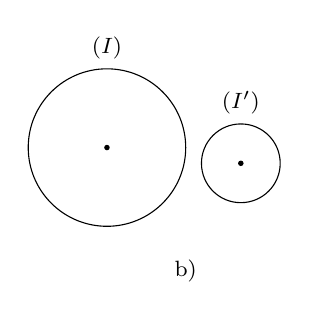
\begin{tikzpicture}[scale=1, font=\footnotesize, line join=round, line cap=round, >=stealth]
		\path
		(0,0) coordinate (I)
		(1.7,-0.2) coordinate (I');
		\draw [samples=200,smooth] (I) circle (1) 
		(I') circle (0.5);
		\draw (1,-1.3) node[below]{b)} (0,1) node[above]{$(I)$} (1.7,0.3) 
		node[above]{$(I')$};
		\foreach \p in{I, I'}
		\fill (\p) circle (1pt);
		
	\end{tikzpicture}
	\hspace{0.8cm}
	%hình c
	\begin{tikzpicture}[scale=1, font=\footnotesize, line join=round, line cap=round, >=stealth]
		\path
		(0,0) coordinate (I)
		(0.6,-1.0) coordinate (I')
		;
		\draw [name path=dgtronI,samples=200,smooth] (I) circle (1); 
		\draw [name path=dgtronI',samples=200,smooth](I') circle 
		(0.65);
		\path[name intersections={of=dgtronI and dgtronI'}]
		(intersection-1) coordinate (B)
		(intersection-2) coordinate (C);
		\draw (-0.1,-1.3) node[below]{c)} (0,1) node[above]{$(I)$} (1.65,-1) 
		node{$(I')$};
		\foreach \p in{I, I'}
		\fill (\p) circle (1pt);
		\foreach \q/\r in{B/-130,C/20}
		\fill (\q) circle (1pt) node[shift={(\r:3mm)}]{$\q$};
	\end{tikzpicture}
	\hspace{0.8cm}
	%hình b
	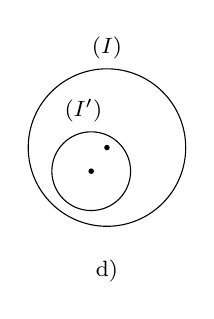
\begin{tikzpicture}[scale=1, font=\footnotesize, line join=round, line cap=round, >=stealth]
		\path
		(0,0) coordinate (I)
		(-0.2,-0.3) coordinate (I');
		\draw [samples=200,smooth] (I) circle (1) 
		(I') circle (0.5);
		\draw (0,-1.3) node[below]{d)} (0,1) node[above]{$(I)$} (-0.3,0.2) 
		node[above]{$(I')$};
		\foreach \p in{I, I'}
		\fill (\p) circle (1pt);
	\end{tikzpicture}
	%		\begin{tikzpicture}
		%			\draw (-2,-2) node[below]{Hình $14$};
		%		\end{tikzpicture}
\end{center}
\loigiai{
\begin{enumerate}
	\item $(I)$ và $(I')$ có đúng một điểm chung, suy ra $(I)$ và $(I')$ tiếp xúc với nhau.
	\item $(I)$ và $(I')$ không có điểm chung, suy ra $(I)$ và $(I')$ không giao nhau. Đồng thời, ta thấy $(I)$ và $(I')$ ở ngoài nhau.
	\item $(I)$ và $(I')$ có đúng hai điểm chung, suy ra $(I)$ và $(I')$ cắt nhau.
	\item $(I)$ và $(I')$ không có điểm chung, suy ra $(I)$ và $(I')$ không giao nhau. Đồng thời, ta thấy $(I)$ đựng $(I')$.
	\end{enumerate}
}
\end{bt}

\begin{bt}%[Dự án EX-9-Đề Cương Toán 9]%[Trần Chiến]%[9H2N1-4]
	Xác định vị trí tương đối của hai đường tròn  $(O; R)$ và $(O'; R')$ trong mỗi trường hợp sau:
	\begin{enumerate}
		\item $OO'=12$; $R=5$; $R'=3$;
		\item $OO'=8$; $R=5$; $R'=3$;
		\item $OO'=7$; $R=5$; $R'=3$;
		\item $OO'=0$; $R=5$; $R'=4$.
	\end{enumerate}
\loigiai{
\begin{enumerate}
	\item Ta có $12>5+3$ nên $OO'>R+R'$, suy ra hai đường tròn $(O;R)$ và $(O';R')$ ở ngoài nhau.
	\item Ta có $8=5+3$ nên $OO'=R+R'$, suy ra hai đường tròn $(O;R)$ và $(O';R')$ tiếp xúc ngoài.
	\item Ta có $5-3<7<5+3$ nên $R-R'<OO'<R+R'$, suy ra hai đường tròn $(O;R)$ và $(O';R')$ cắt nhau.
	\item Ta có $0<5$ nên $OO'<R-R'$, suy ra đường tròn $(O;R)$ đựng đường tròn $(O';R')$.
\end{enumerate}
}
\end{bt}